\documentclass{beamer}
\usepackage[absolute,overlay]{textpos}
\usepackage{pifont}
\setbeamertemplate{bibliography item}[text]
\setbeamertemplate{navigation symbols}{}
\setbeamertemplate{caption}[numbered] 
\setbeamerfont{caption}{size=\scriptsize}
\setbeamertemplate{footline}[frame number]

\setbeamerfont{page number in head/foot}{size=\large}
\setbeamertemplate{footline}[frame number]

\usepackage{units}
\usepackage{amssymb}
\usepackage{color}
\definecolor{offyellow}{cmyk}{0, 0, 1, .2}
\usepackage{movie15}

\newcommand\FrameText[1]{
\begin{textblock}{16}(1,2.5)
\raggedright #1
\end{textblock}}

\begin{document}

\addtobeamertemplate{frametitle}{}{
\begin{textblock}{16}(0,0)

\includegraphics[scale=0.5]{Header.png}
\end{textblock}}

\begin{frame}
\frametitle{1}
\begin{picture}(0.0,0.0)
\put(-28.45,-142){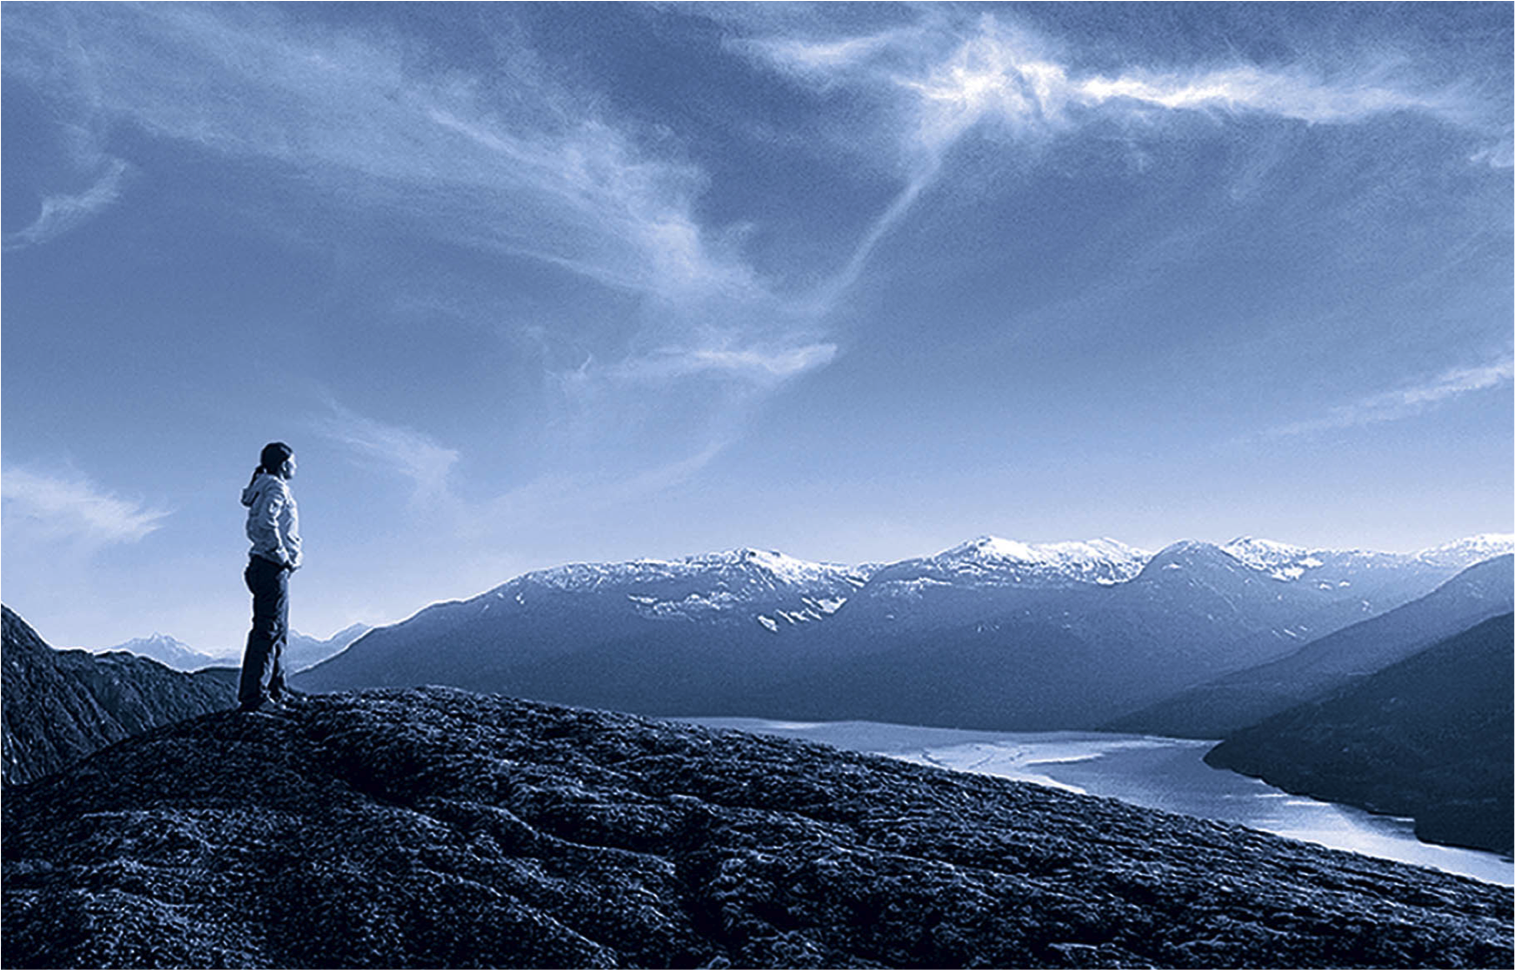
\includegraphics[width=\paperwidth]{FrontPage.png}}
\end{picture}
\FrameText{
\textcolor{white}{\bf{\LARGE The Effects of two Parameters on idealized Convective Boundary Layer Entrainment}}\\
\textcolor{white}{\bf{\LARGE M.Sc. Defense}}\\
\textcolor{white}{\bf{Niamh Chaparro}}}
\end{frame}

\begin{frame}
\frametitle{2}
%\FrameText{what is the convective boundary layer and its entrainment zone}
The atmospheric convecitive boundary layer starts to grow over land shortly\\
sunrise when the sun warms the surface and thermals start to form and rise.\\
The thermals impinge on the air above which is at a stable lapse rate, ie\\
the potential temperature increases with altitude and sometimes has an inversion.\\
So they recoil or overturn, depending on how strong the inversion or stability is
and concurrently drag stable air into the growing mixed layer.  this is called\\
entrainment and is how the convective boundary layer or CBL grows\\ 
The convective boundary layer or CBL is made up of a surface layer\\
which we don't really care about in this context, a turbulent well\\
mixed layer where potential temperature and tracer concentrations are almost uniform\\
an entrainment zone where entrainment is initiated by overturnig or recoil of thermals.\\
and then above is the free atmosphere.\\

\end{frame}


\begin{frame}
\frametitle{3}
We study CBL entrainment becuse CBL height is needed to calculate\\
CBL concentrations of anything.  Knowledge of entrainment zone \\
depth enables cumulous cloud cover calculations and parametrizations\\
for both are neede in global circulation models.\\
\end{frame}

\begin{frame}
This topic has been studied for over 30 years and there three types\\
of studies:  those using measurement, those using numerical models\\
that solve the navier stokes equations on a discrete grid such as\\
large eddy simulation and direct numerical simulation\\
and those using bulk models with are simpler numerical models\\
based on average quantities and simplified profiles\\
usually each one refers to at least one of the other types\\
and my study falls into the second category, ie its an LES study.
\end{frame}

\begin{frame}
So this topic has been studied for over 30 years and a broad\\
understanding has been established but there is ongoing discussion\\
about the degree of discrete resolution required to capture CBL\\
entrainmnet, the multitude of definitions of entrainment zone and\\
CBL height definitions and the forms of the relationships of\\
entrainment rate, and entrainment zone depth to convective\\
richardson number, which i'll define later and which represents\\
the forcings at the entrainment zone.

\end{frame}


\begin{frame}
I set out to model the dry idealized CBL in the absence of large\\
scale winds and applied higher resolution than used in the 
other comparable studies.  This decision was influenced by a 2011 resolution\\
study by patton and sullivan who showed that the shapes of the profiles\\
within the entrainment zone are sensitive to grid size.\\
I based my height defintions on the potential temperature profile\\
because it represents the thermodynamic state of the CBL as well\\
as its three layer structure, and it hasn't been used before for this\\
purpose.  And I examine the resulting relationships of entrainemnt rate\\
and entrainment zone depth to convective richardson number.  
\end{frame}


\begin{frame}
I used the System for Atmospheric Modelling which is an LES\\
desigened to resolve clouds.  So it uses the anelastic equations\\
of motion to take into consideration density changes that occur\\
over the required modeled depth, for deep convection.\\
The prognosed thermodynamcial variabe is liquid ice static\\
energy and potential temperature is then diagnozed.  Subgrid\\
viscosity and fluxes are modeled using first order Smagorinski\\
closure and scalars are advected using a 3d positive definite\\
scheme to minimise numerical diffusion.\\
\end{frame}

\begin{frame}
I carried out 7, 10 ensemble runs varying the two principal external parameters\\
Surfance heat flux and upper stable lapse rate. One of them was a mistake
\end{frame}

\begin{frame}
Now for my definitions.\\
on the left is potential temperature profile and in the middle\\
is its vertical gradient.  I define CBL height as the point\\
of maximum gradient, the lower ez boundary as the point where\\
the gradient significantly exeeds zero and the upper ez boundary\\
as the point at which the gradient resumes the upper lapse rate\\
gamma\\
on the right is the heat flux profile, which is usually used\\
in modelling studies to define the CBL height and EZ limits\\
and you can see the heights are different.\\
\end{frame}

\begin{frame}
So h is the CBL height ie the point of maximum potential temperature gradient\\
the mixed layer temperature is the average over the layer, the dearforff\\
velocity scale is based on the surface heat flux and effective scales\\
the turbulent velocities in the CBL.  the potential temperature jump\\
i define as the difference accross the entrainment zone.  and the convective\\
richardson uses these variables, and is a ratio of the convective momentum\\
and the bouyancy which acts to suppress it, in the entrainment zone.

\end{frame}

\begin{frame}
Heres a visualization from one of the runs.  It's a vertical cross\\
section of potential temperature.  Darker shading represents air \\
at potential temperature close to the mixed layer average.  lighter\\
represents warmer.  Thermals form and rise.  they impinge and recoil\\
This is a high stability run, so at if it were lower, you would see\\
freeer motion at the top, so more overturning.  Regardless, warmer\\
air is dragged down from the top.\\

\end{frame}

\begin{frame}
The entrainment zone can be thought of as the local region over which\\
a profile goes transitions from mixed layer to free atmospheric characteristics.\\
or the horizontal variation of local CBL height.  So now I'll consider the latter\\
here is a local potential temperature profile where the height is relatively low\\
i fit three lines to the profile representing the mixed layer the entrainment zone\\
and the free atmosphere.  and then looked at their distributions.\\
\end{frame}

\begin{frame}
So here on the left the lapse rate is the same but the surface heat\\
flux goes from 60 to 150.  lighter shading represents lower heat flux\\
overall height and its variance increases with increasing surface heat flux.\\
but when the heights are scaled by h (point of average maximum gradient)\\
the distributions become more similar.  for runs at lower surface heat flux\\
there are relatively fewer bins, and higher counts in each bin so u can imagine\\
if there were infinite bins, perhaps the distributions would become even more similar\\
i dunno.  anyway look at the limits.  as gamma decreases.
\end{frame}

\begin{frame}
the top limit remains between 1 and 1.2
\end{frame}

\begin{frame}
but the bottom limit decreases.
\end{frame}

\begin{frame}
\end{frame}



\begin{frame}
so the lower limit or entrainment zone boundary increases with increased stability\\
resulting in a narrower scaled entrainment zone.
\end{frame}

\begin{frame}
Now lets look at the entrainment zone based on the average profiles.\\
on the right, average potential temperature increases in time.   its\\
vertical gradient in the middle represents the growing CBL\\
with its three layer structure\\
as does the heat flux profile which represents the vertical\\
mixing of turbulent temperature fluctuations that cause warming\\
\end{frame}

\begin{frame}
To define the lower entrainment zone boundary based on the vertical\\
potential temperature gradient i chose a threshold\\
value which was small positive, the same for all runs and an order\\
of magnitude less than the upper lapse rate.\\
\end{frame}

\begin{frame}
the resulting scaled entrainment zone depth narrows in time and with increased\\
stability mostly due to an increase in the lower scaled entrainment zone boundary\\
richardson number is a measure of stability, and increases in time for all runs\\
\end{frame}

\begin{frame}
so the scaled lower ez boundary increases with increasing richardson number\\
\end{frame}


\begin{frame}
so now look at the relationship of the scaled entrainment zone depth to richardson numver\\
we see it decreases with increased richardson number, the xaxis is one over the richardson\\
number.\\
the curves group according to upper lapse rate\\
\end{frame}

\begin{frame}
curves representing the relationship of scaled entrianment zone\\
depth to richardson numer group by gamma
\end{frame}

\begin{frame}
if i define my heights based on the average vertical potiential temperature gradient\\
scaled by gamma on the right here.\\
\end{frame}

\begin{frame}
the order of the limits switch.  ie the runs at higher stability, represented by the\\
triangles have lower entrainment zone limits that are lower when based on the \\
gradient, but higher when based on the scaled gradient.
\end{frame}

\begin{frame}
this causes the curves representing the relationship of scaled entrainment\\
zone depth to richardson number to collapse\\
\end{frame}

\begin{frame}
so the curves representing the relationship of scaled entrainment zone depth\\
to richardson number group according to gamma when heights are based on the\\
average vertical potential temperature gradient, but collapse when heights\\
are based on the scaled average vertical potential temperature gradient.
\end{frame}

%\begin{frame}
%\frametitle{25}
%\FrameText{The downward moving warm potential temperature fluctuations ($\theta^{'+}_{h} \ where w^{'}<0$) at $h$ ``warms'' the air below
%}
%\end{frame}

\begin{frame}
so the gradient in the upper cbl is scaled by the upper lapse rate.  this must be related\\
to the downward moving warm air above, say at h.  so lets look at that.  so, we have\\
thermals of varying heights impinging on the free atmosphere.  and this horizontal\\
variance in height represents the entrainment zone.  in the entrainmnent zone\\
much of the air is at the initial or background lapse rate gamma.  so if this air\\
is brought down from the top of the entrainmnet zone to h, the resulting difference\\
between its potential temperature and that of the surrounding air at h is delta h times\\
gamma. 
\end{frame}


\begin{frame}
based on the plots here of the downward moving positive potential temperature fluctuations\\
at h, delta h times gamma seems to be a effective scale. ie the plot on the right
\end{frame}


\begin{frame}
so the downward moving positive temperature fluctuations at h are scaled by or depend on gamma
\end{frame}

\begin{frame}
back to the relationship of scaled entrainment zone depth to richardson number.  plotting it\\
in log log coordinates shows that it has an exponent that is predicted by theory and\\
seen in other similar studies.  also it seems to change with increased richardson numver\\
which hasn't been explicitly pointed out before\\
\end{frame}

\begin{frame}
the relationship of scaled entrainment rate to richardson number also has exponent\\
in line with theory and other studies, and seems to change wrt richardson number\\
that seem to change as richardson number increases
\end{frame}

\begin{frame}
so the scaled entrainment zone decreases with increasing richardson number\\
the potential temperature gradients in the upper cbl and the positive\\
downward moving flucutuationns at h depend on gamma\\
ther is a change in entrainment regime as richardson number increases\\
and entrainmnet zone boundary defintions based on the scaled average\\
vertical potential temperature gradient are valid.
\end{frame}

\begin{frame}
\frametitle{2}
\FrameText{\bf{\large References}}
\begin{thebibliography}{99}
\bibitem{SullPat} Peter P. Sullivan and Edward G. Patton 2011: \emph{The Effect of Mesh Resolution on Convective Boundary Layer Statistics and Structures Generated by Large Eddie Simulation}. Journal of the Atmospheric Sciences, 58, 2395-2415.
\bibitem{Stull-BLMetIntro} Roland Stull 1988: \emph{An Introduction to Boundary Layer Meteorology}. Kluwer Academic Publishers.

\end{thebibliography}
\end{frame}


\end{document}


